\documentclass[sigconf,review,anonymous]{acmart}

\AtBeginDocument{%
  \providecommand\BibTeX{{%
    Bib\TeX}}
}
\usepackage{tikz}
\usetikzlibrary{arrows.meta,positioning,fit}

\setcopyright{none}
\acmConference[CHI '27]{Proceedings of the 2027 CHI Conference on Human Factors in Computing Systems}{April 2027}{Yokohama, Japan}
\acmBooktitle{CHI '27: Proceedings of the 2027 CHI Conference on Human Factors in Computing Systems}
\acmDOI{TBD}
\acmISBN{TBD}

\begin{document}

\title{VibeRobot!: Vibe-to-Verify End-User Programming for Robot Arms}

\begin{abstract}
Natural-language task authoring is making robot programming accessible to non-experts, but practical success still breaks at the same point: after first-generation plans fail. In our iterative development of \textbf{VibeRobot}, users repeatedly hit a failure pattern of opaque errors, weak context carryover across retries, and unclear control boundaries between preview and execution. We present \textbf{ArmCraft}, a \emph{Vibe-to-Verify} interaction design that treats robot vibe coding as a verification loop rather than a one-shot generation problem. ArmCraft combines (1) task-spec normalization from natural language, (2) simulation-first gating with explicit user approval before movement, (3) novice-oriented failure cards that expose where and why plans fail, and (4) constrained patch suggestions for low-friction repair. We contribute an implementation-grounded architecture, a sharpened research agenda on performance/learning/attribution, and a CHI-oriented mixed-method evaluation plan. The core claim is that better robot end-user development requires UX for debugging, safety, and accountability, not only stronger planners.
\end{abstract}

\begin{CCSXML}
<ccs2012>
<concept>
<concept_id>10003120.10003121.10003122</concept_id>
<concept_desc>Human-centered computing~Human computer interaction (HCI)</concept_desc>
<concept_significance>500</concept_significance>
</concept>
<concept>
<concept_id>10003120.10003130.10011762</concept_id>
<concept_desc>Human-centered computing~Empirical studies in HCI</concept_desc>
<concept_significance>500</concept_significance>
</concept>
<concept>
<concept_id>10010147.10010919.10010172</concept_id>
<concept_desc>Computing methodologies~Robotic planning</concept_desc>
<concept_significance>300</concept_significance>
</concept>
</ccs2012>
\end{CCSXML}

\ccsdesc[500]{Human-centered computing~Human computer interaction (HCI)}
\ccsdesc[500]{Human-centered computing~Empirical studies in HCI}
\ccsdesc[300]{Computing methodologies~Robotic planning}

\keywords{robot end-user development, LLM, simulation-first verification, interactive debugging, human-AI collaboration, responsibility attribution}

\maketitle

\section{Introduction}
Language-first robot interfaces are improving rapidly through LLM-based planning and control systems such as SayCan, Inner Monologue, ProgPrompt, Code as Policies, VoxPoser, PaLM-E, and RT-2~\cite{ahn2022saycan,huang2022innermonologue,singh2022progprompt,liang2023codeaspolicies,huang2023voxposer,driess2023palme,brohan2023rt2}. Quantitatively, this line already reports large-scale capability signals (e.g., RT-2 evaluation over 6k trials, and PaLM-E instantiated at 562B parameters)~\cite{brohan2023rt2,driess2023palme}. In parallel, early end-user systems now show that non-experts can produce useful robot apps with LLM support~\cite{karli2024alchemist,ge2024cocobo}. This shift makes ``natural language to robot behavior'' feasible, but not yet reliable in novice workflows.

Our formative QA and engineering triage in VibeRobot indicate a consistent bottleneck: generation is easy; \emph{failure recovery} is hard. Users can issue follow-up corrections (e.g., ``not that one,'' ``do it properly''), but systems may lose context, produce under-specified plans, or execute with weak transparency. This motivates three practical risks we explicitly design for: low success under iteration, weak safety confidence, and unstable responsibility attribution when outcomes fail.

We frame this as an HCI systems problem, not only a model-quality problem. ArmCraft therefore proposes a \textbf{Vibe-to-Verify} loop: users can ask in plain language, but every execution must pass simulation preview and explicit approval; failures are translated into novice-readable diagnosis; patch suggestions are small, actionable, and immediately testable.

\subsection{Contributions}
This paper contributes:
\begin{itemize}
  \item \textbf{C1 (Design)}: ArmCraft, an interaction architecture for robot end-user development that integrates sim-first approval, failure inspection, and patch-based repair.
  \item \textbf{C2 (Implementation)}: A running prototype that operationalizes ArmCraft with end-to-end stages from intent extraction to approval-gated execution and iterative retries.
  \item \textbf{C3 (Research Agenda)}: A CHI-oriented evaluation design with explicit hypotheses across productivity, transfer learning, explanation uptake, trust calibration, and responsibility attribution.
  \item \textbf{C4 (Methodological Bar)}: A reproducibility plan (structured logs, analysis preregistration, artifact release) aimed at rigorous systems+user-study evidence.
\end{itemize}

\section{Related Work}
\subsection{LLM-Based Robot Planning and Embodied Control}
Recent work demonstrates broad capability gains in language-conditioned robot behavior: affordance-aware skill selection~\cite{ahn2022saycan}, explicit language-mediated reasoning loops~\cite{huang2022innermonologue}, code-generation-based policy construction~\cite{liang2023codeaspolicies}, language-to-plan synthesis~\cite{singh2022progprompt}, multimodal embodied models~\cite{driess2023palme,brohan2023rt2}, and compositional spatial value maps~\cite{huang2023voxposer}. Code as Policies also reports a 39.8\% HumanEval score under hierarchical code generation, showing stronger program synthesis capacity behind embodied control logic~\cite{liang2023codeaspolicies}. However, these systems primarily optimize planning and execution quality, while user-facing debugging and accountability workflows remain under-specified.

\subsection{Robot End-User Development}
Longstanding robot EUD literature emphasizes teaching aids, demonstration interfaces, and low-code authoring for non-programmers~\cite{alexandrova2014pbd,ajaykumar2021kinesthetic,fogli2022hybrid}. Newer LLM-mediated systems (e.g., Alchemist~\cite{karli2024alchemist}, Cocobo~\cite{ge2024cocobo}) reduce authoring friction further. Yet, a persistent gap is \emph{iterative failure repair}: novice users still need support to interpret failure causes, choose safe corrections, and verify improvements before real motion.

\subsection{Actionable Explanations and Explanatory Debugging}
HCI and IUI research has established that explanations are useful only when they support user action~\cite{kulesza2015principles,kulesza2013too}. Broader XAI work in HCI similarly emphasizes explanation utility, accountability, and user experience~\cite{abdul2018trends,liao2020questioning}. ArmCraft adapts this line to embodied task execution by binding explanations directly to corrective patches and immediate re-simulation.

\subsection{Trust Calibration and Responsibility Attribution}
Human factors work shows that trust in automation should be calibrated to system capability, not blindly increased~\cite{lee2004trust,parasuraman1997humans,hancock2011meta}. A quantitative anchor is Hancock et al.'s HRI trust meta-analysis: 29 studies, with aggregate effect sizes of $\bar{r}=0.26$ (correlational) and $\bar{d}=0.71$ (experimental)~\cite{hancock2011meta}. In robot vibe coding, trust calibration and attribution are tightly coupled: users decide whether failure is ``my instruction,'' ``the robot,'' or ``the AI planner.'' Existing robot programming interfaces rarely expose this attribution dynamic as a primary design objective.

\begin{table}[t]
  \caption{Selected quantitative signals from prior work that motivate ArmCraft.}
  \label{tab:prior-quant}
  \begin{tabular}{p{2.0cm}p{5.0cm}}
    \toprule
    Work & Quantitative signal \\
    \midrule
    RT-2 & Reports evaluation over 6k robotic trials~\cite{brohan2023rt2}. \\
    PaLM-E & Instantiates an embodied multimodal model at 562B parameters~\cite{driess2023palme}. \\
    Code as Policies & Reports 39.8\% on HumanEval via hierarchical code generation~\cite{liang2023codeaspolicies}. \\
    HRI trust meta-analysis & Synthesizes 29 studies with aggregate effects $\bar{r}=0.26$, $\bar{d}=0.71$~\cite{hancock2011meta}. \\
    \bottomrule
  \end{tabular}
\end{table}

\subsection{Gap Summary}
The literature strongly covers language-to-robot generation and general explainability principles. The open CHI opportunity is the \textbf{interaction loop from failure to verified repair} for novices, with measurable effects on learning transfer, control, and attribution. ArmCraft targets that gap.

\section{ArmCraft: Vibe-to-Verify Architecture}
Figure~\ref{fig:system-overview} shows the full architecture as implemented in our prototype and extended for CHI evaluation.

\begin{figure*}[t]
  \centering
  \resizebox{\textwidth}{!}{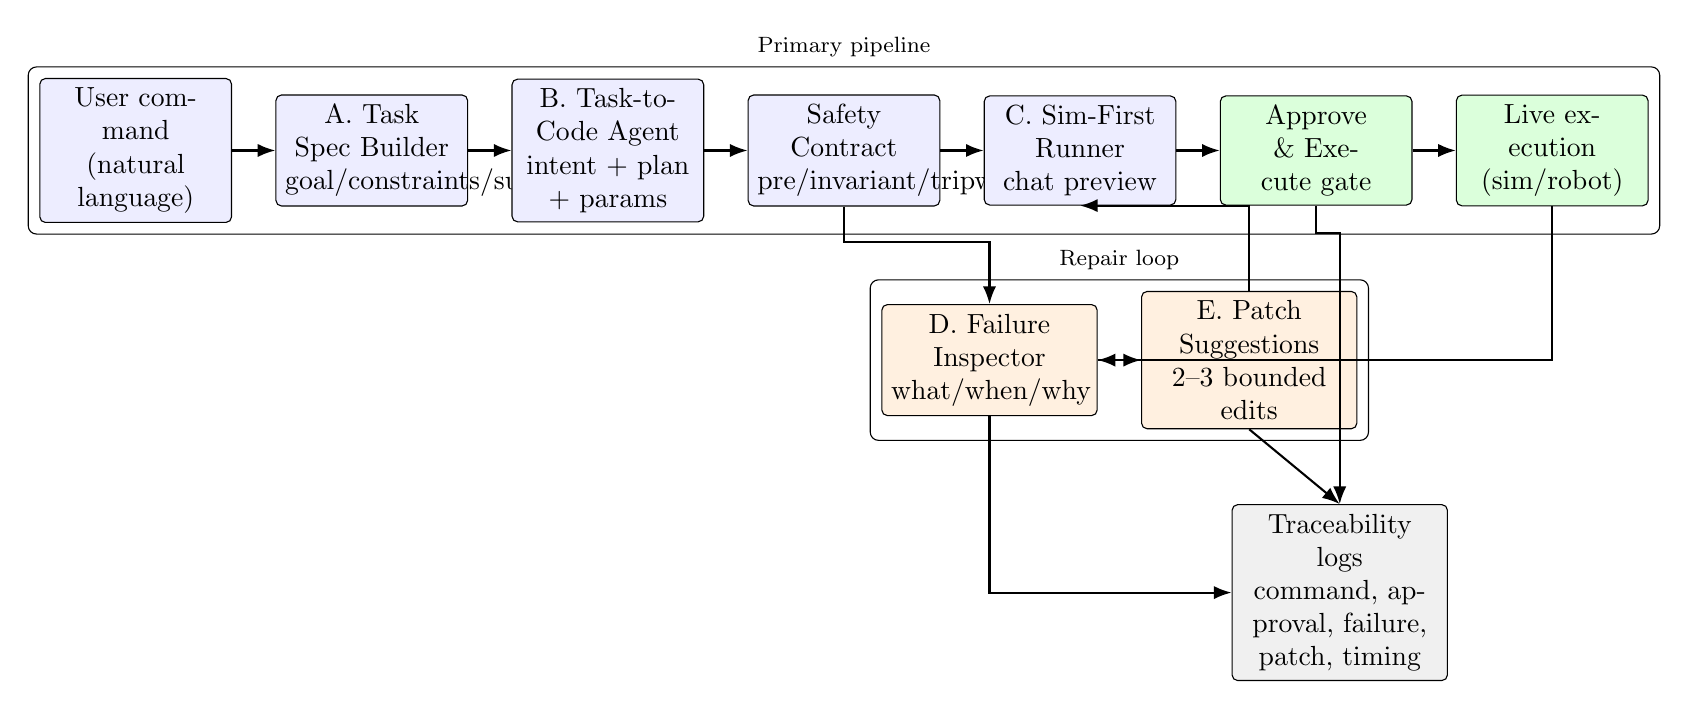
\begin{tikzpicture}[
  x=1cm,
  y=1cm,
  node distance=0.55cm and 0.55cm,
  module/.style={draw, rounded corners=2pt, align=center, minimum height=1.0cm, text width=2.2cm, fill=blue!7},
  support/.style={draw, rounded corners=2pt, align=center, minimum height=0.95cm, text width=2.5cm, fill=orange!12},
  gate/.style={draw, rounded corners=2pt, align=center, minimum height=1.0cm, text width=2.2cm, fill=green!14},
  trace/.style={draw, rounded corners=2pt, align=center, minimum height=0.85cm, text width=2.5cm, fill=gray!12},
  arr/.style={-Latex, line width=0.75pt}
]

\node[module] (user) {User command\\(natural language)};
\node[module, right=of user] (spec) {A. Task Spec Builder\\goal/constraints/success};
\node[module, right=of spec] (plan) {B. Task-to-Code Agent\\intent + plan + params};
\node[module, right=of plan] (safe) {Safety Contract\\pre/invariant/tripwire};
\node[module, right=of safe] (preview) {C. Sim-First Runner\\chat preview};
\node[gate, right=of preview] (approve) {Approve\\\& Execute gate};
\node[gate, right=of approve] (exec) {Live execution\\(sim/robot)};

\node[support, below=1.25cm of preview, xshift=-1.15cm] (inspect) {D. Failure Inspector\\what/when/why};
\node[support, right=of inspect] (patch) {E. Patch Suggestions\\2--3 bounded edits};
\node[trace, below=0.95cm of patch, xshift=1.15cm] (audit) {Traceability logs\\command, approval, failure, patch, timing};

\draw[arr] (user) -- (spec);
\draw[arr] (spec) -- (plan);
\draw[arr] (plan) -- (safe);
\draw[arr] (safe) -- (preview);
\draw[arr] (preview) -- (approve);
\draw[arr] (approve) -- (exec);

\draw[arr] (exec.south) |- (inspect.east);
\draw[arr] (inspect) -- (patch);
\draw[arr] (patch.north) |- (preview.south);
\draw[arr] (safe.south) -- ++(0,-0.45) -| (inspect.north);
\draw[arr] (approve.south) -- ++(0,-0.35) -| (audit.north);
\draw[arr] (inspect.south) |- (audit.west);
\draw[arr] (patch.south) -- (audit.north);

\node[draw, rounded corners=3pt, fit=(user)(exec), inner sep=4pt, label={[font=\footnotesize]above:Primary pipeline}] {};
\node[draw, rounded corners=3pt, fit=(inspect)(patch), inner sep=4pt, label={[font=\footnotesize]above:Repair loop}] {};

\end{tikzpicture}
}
  \caption{ArmCraft architecture mapped to the running prototype. Execution is blocked until simulation preview and explicit user approval succeed.}
  \Description{LaTeX-native framework diagram from user command through task specification, planning, safety, preview, approval, execution, and failure-repair loop.}
  \label{fig:system-overview}
\end{figure*}

\subsection{Design Requirements}
ArmCraft is driven by three requirements derived from repeated QA and user-facing failures:
\begin{itemize}
  \item \textbf{R1: Controllability}. No robot motion without explicit approval after preview.
  \item \textbf{R2: Repairability}. Failures must be translated into reasons and concrete next actions.
  \item \textbf{R3: Accountability}. System transitions and safety constraints must be inspectable and auditable.
\end{itemize}
These requirements are aligned with prior human-AI interaction guidance on user control, feedback, and trust calibration~\cite{amershi2019guidelines,lee2004trust}.

\subsection{Five Fixed Modules}
\textbf{A. Task Spec Builder}. Natural language is normalized into explicit slots (goal, targets, constraints, success criteria, assumptions) to avoid downstream ambiguity.

\textbf{B. Task-to-Code Agent}. The planner emits \emph{code + test intent + execution constraints} rather than code alone, enabling verification and post-hoc analysis.

\textbf{C. Sim-First Runner}. UI transition is strictly \texttt{Simulate -> Approve \& Execute}. Pre-approval simulation is visible in chat preview; the execution view remains non-moving until approval.

\textbf{D. Failure Inspector}. Failures are summarized as cards with type, time slice, and causal cues (e.g., collision overlap, unstable grasp, unreachable pose, workspace violation).

\textbf{E. Patch Suggestions}. The system proposes 2--3 bounded edits (e.g., top-down regrasp, speed cap, path replan, target lock) to reduce decision fatigue and accelerate retry.

\begin{figure}[t]
  \centering
  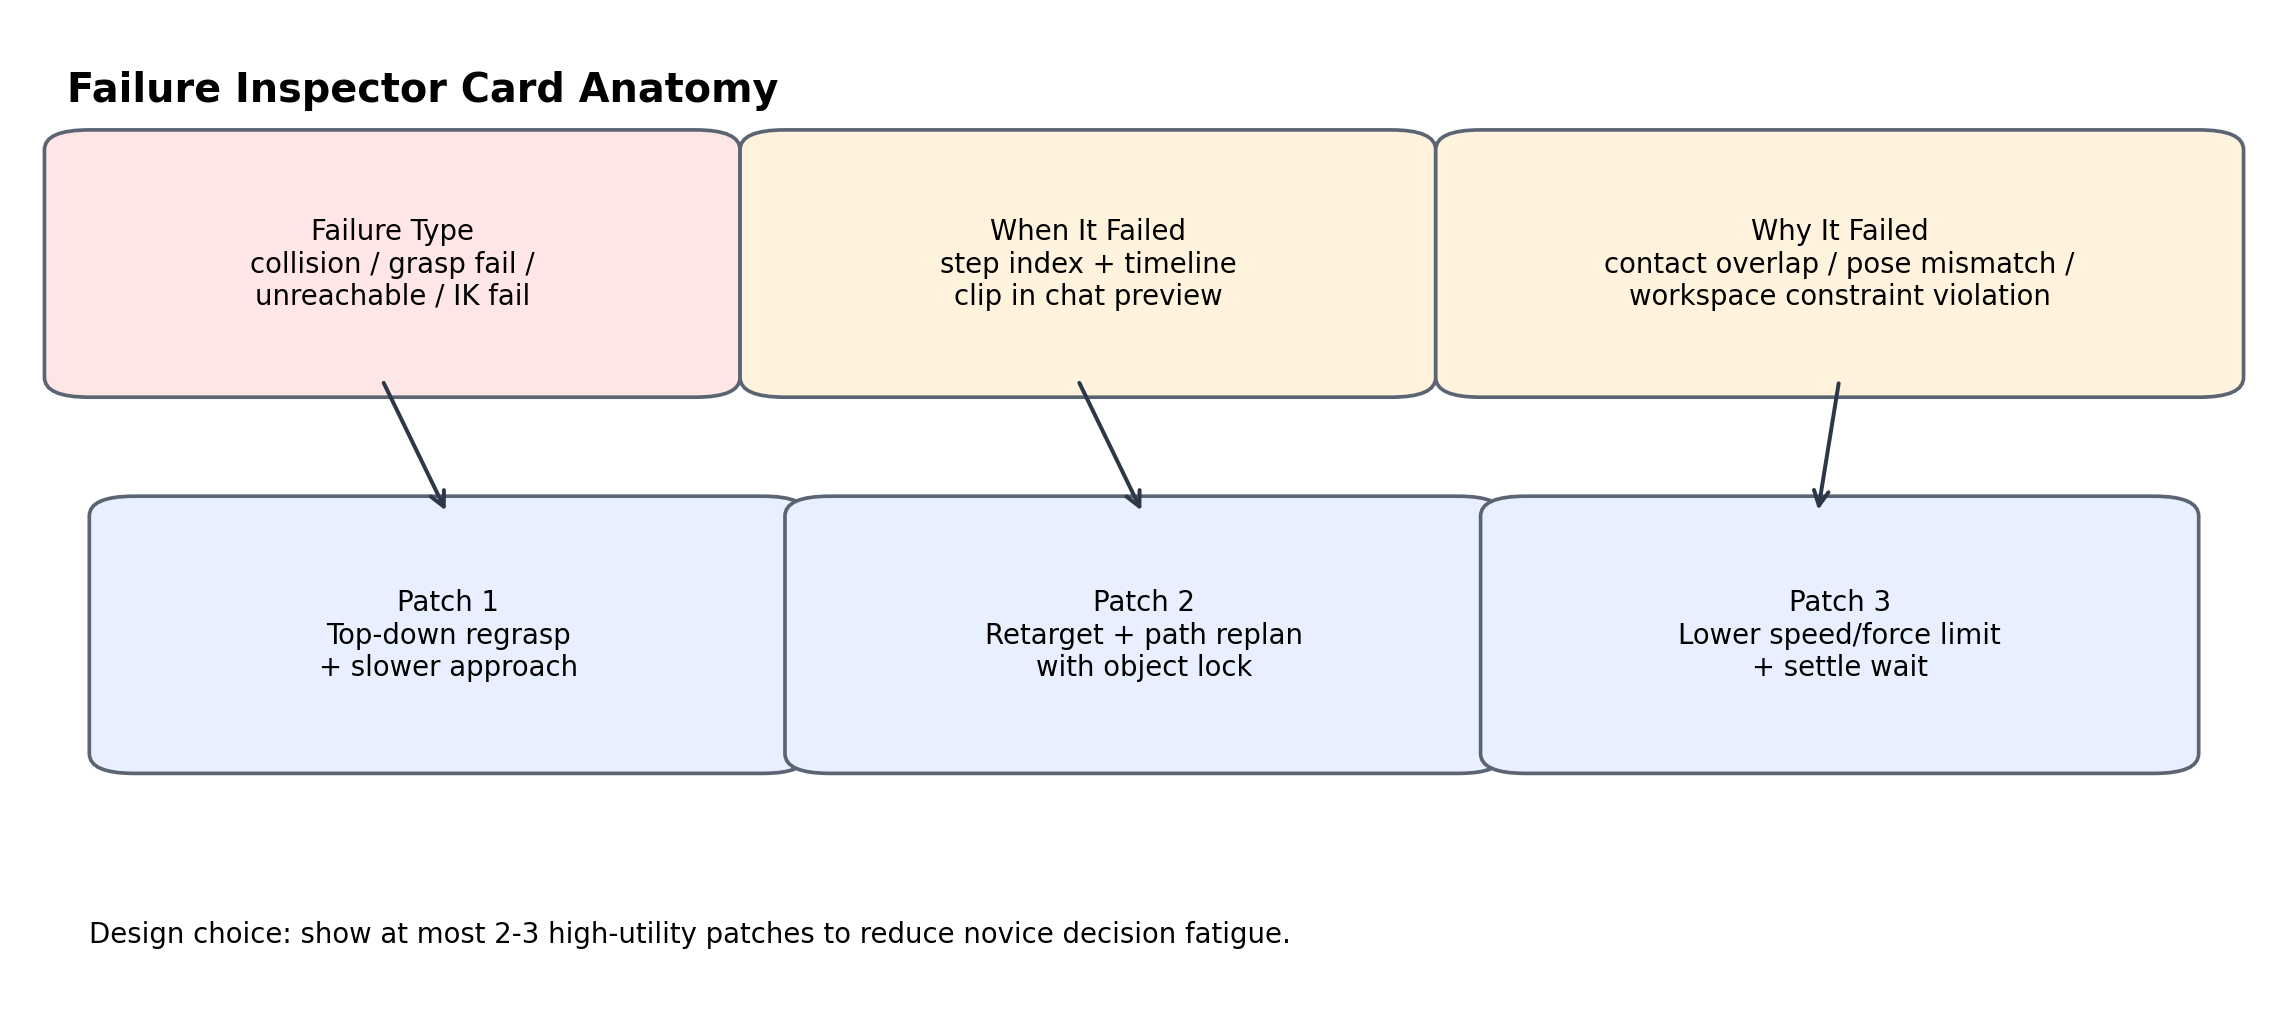
\includegraphics[width=\columnwidth]{figures/failure_inspector.png}
  \caption{Failure Inspector structure in ArmCraft: what failed, when it failed, why it failed, and a short patch set for immediate re-simulation.}
  \Description{Diagram of failure card anatomy with three card sections and three example patch suggestions.}
  \label{fig:failure-inspector}
\end{figure}

\subsection{Loop-Level Interaction}
Figure~\ref{fig:interaction-loop} summarizes the user loop.

\begin{figure}[t]
  \centering
  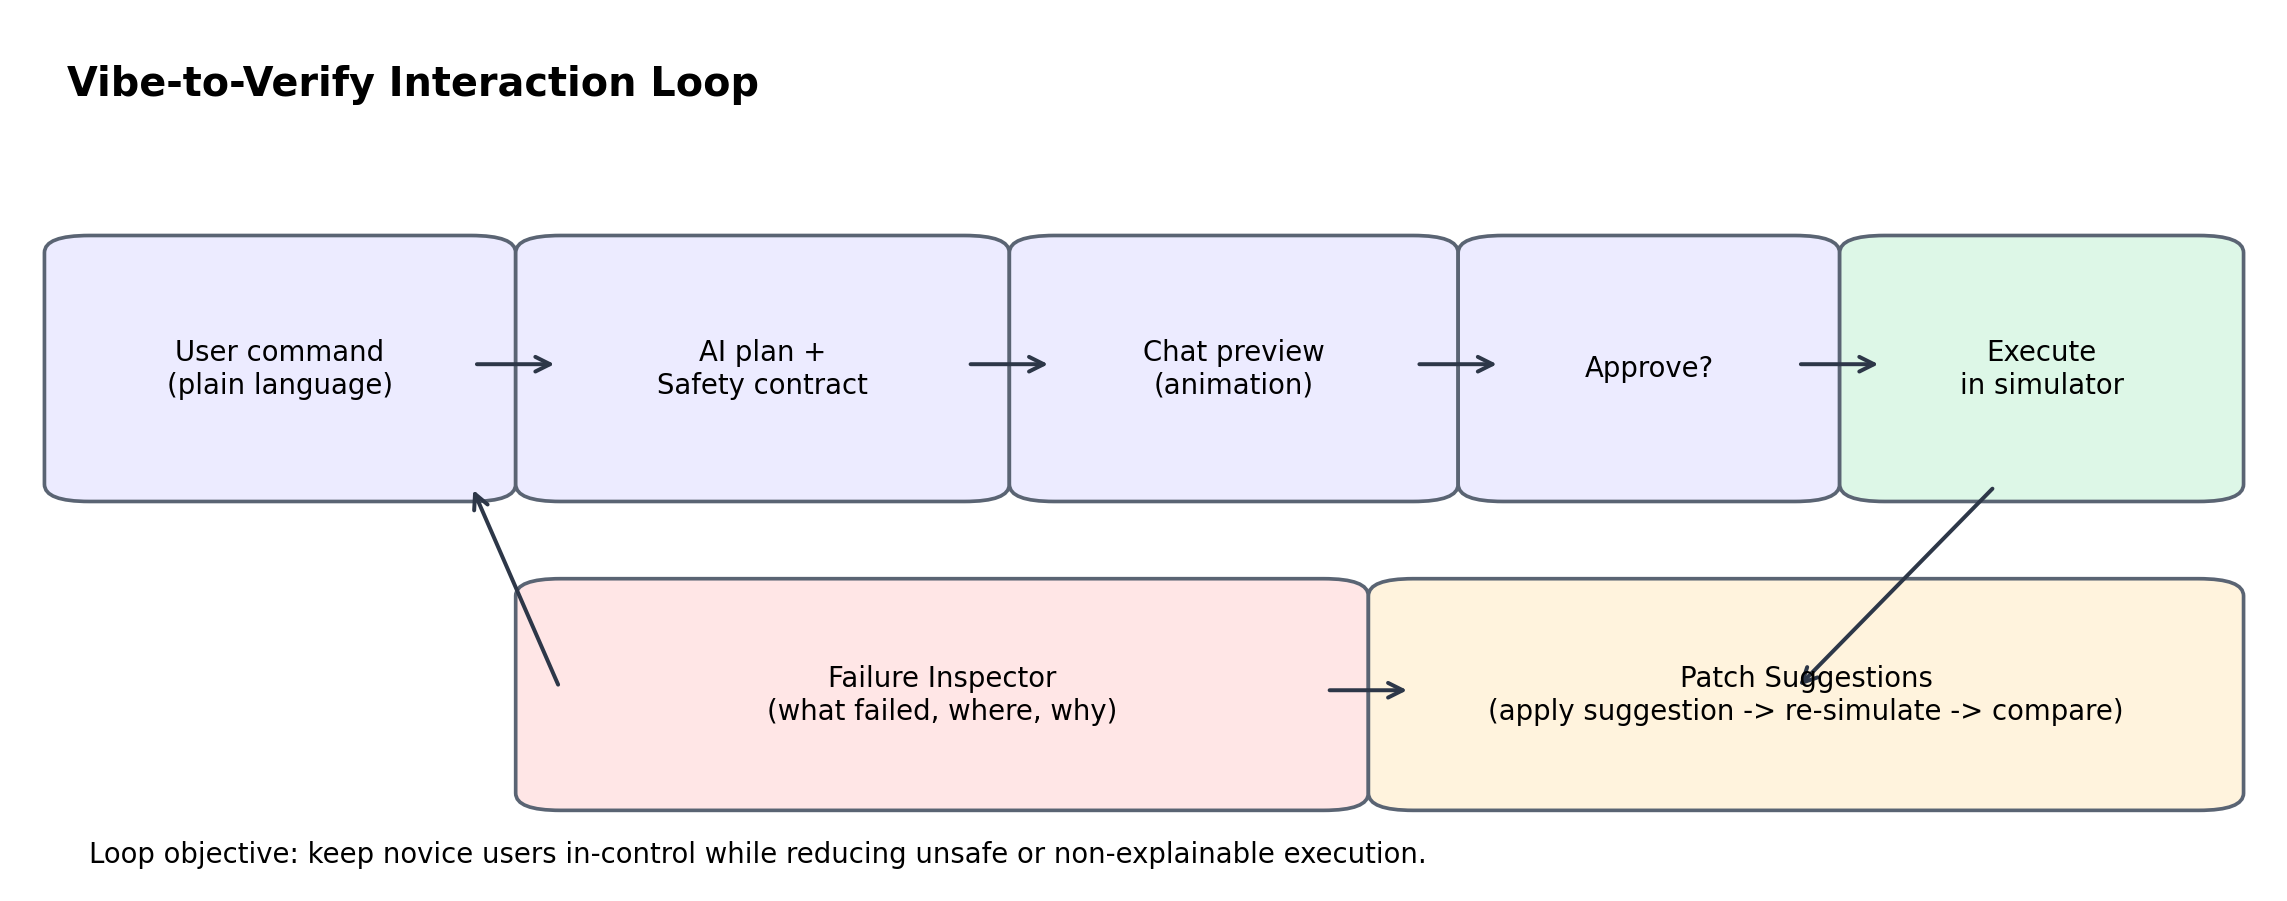
\includegraphics[width=\columnwidth]{figures/interaction_loop.png}
  \caption{Vibe-to-Verify interaction loop. The user remains in control through explicit approval and patch-guided repair.}
  \Description{Flow from command to plan/preview, approval, execution, then failure inspector and patch suggestions looping back.}
  \label{fig:interaction-loop}
\end{figure}

\subsection{Pipeline Hardening from QA}
We incorporated concrete hardening updates motivated by observed failure cases:
\begin{itemize}
  \item \textbf{Semantic-to-executable normalization}: repairs under-specified action parameters before execution.
  \item \textbf{Retry-context target lock}: keeps object references stable across corrective follow-ups.
  \item \textbf{Scene isolation}: deep-copy scene presets to prevent cross-session state contamination.
  \item \textbf{Approval-state enforcement}: simulation and execution channels remain explicitly separated until user consent.
\end{itemize}

\section{Research Questions and Hypotheses}
\textbf{RQ1 (Performance and Learning).} Does ArmCraft increase novice task success and transfer to perturbed scenes?

\textbf{RQ2 (Comprehension-to-Action).} Which failure representations most effectively drive correct next-step actions?

\textbf{RQ3 (Attribution and Trust).} How does ArmCraft shift responsibility attribution and trust calibration under repeated failure-repair cycles?

We operationalize these with directional hypotheses:
\begin{itemize}
  \item \textbf{H1}: ArmCraft reduces time-to-first-success and iterations vs. Vibe-only and Sim-first-only baselines.
  \item \textbf{H2}: ArmCraft improves transfer success under object-position perturbations.
  \item \textbf{H3}: ArmCraft reduces workload and increases perceived control without inflating blind trust.
  \item \textbf{H4}: ArmCraft produces more calibrated attribution (less default self-blame or agent-blame) by exposing failure causality.
\end{itemize}

\section{Evaluation Plan}
Figure~\ref{fig:study-design} outlines the two-study program.

\begin{figure}[t]
  \centering
  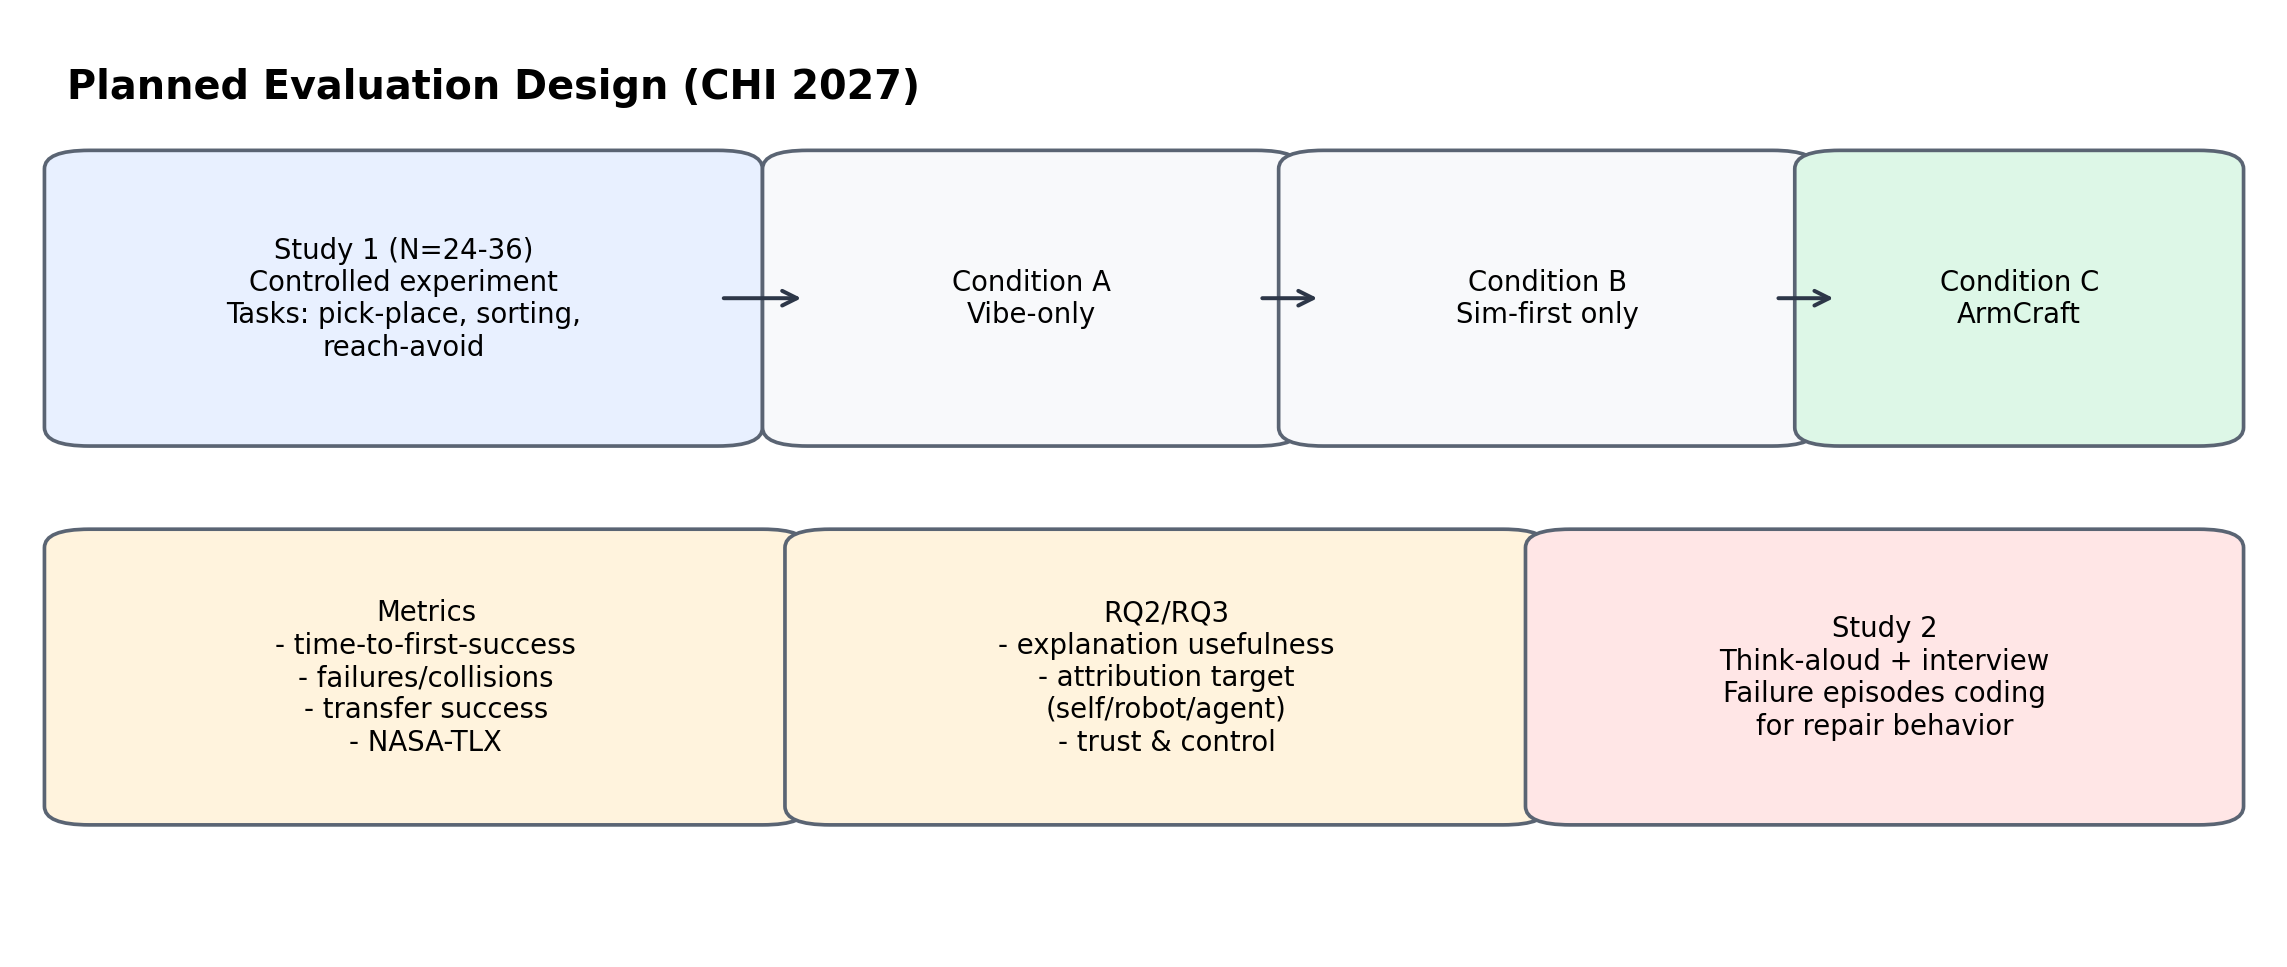
\includegraphics[width=\columnwidth]{figures/study_design.png}
  \caption{Planned CHI evaluation: controlled experiment (Study 1) plus qualitative deep dive (Study 2).}
  \Description{Diagram of three-condition experiment and think-aloud interview follow-up.}
  \label{fig:study-design}
\end{figure}

\subsection{Study 1: Controlled Experiment (N=24--36)}
\textbf{Conditions.}
\begin{itemize}
  \item \textbf{Vibe-only}: natural language plan generation + direct simulation execution.
  \item \textbf{Sim-first only}: forced preview/approval but raw logs (no Failure Inspector/Patches).
  \item \textbf{ArmCraft}: full loop with inspector and patch suggestions.
\end{itemize}

\textbf{Tasks.}
Pick-and-place, sorting, and reach-avoid tasks under standardized scenes and perturbation trials.

\begin{table}[t]
  \caption{Condition features in Study 1.}
  \label{tab:conditions}
  \begin{tabular}{lccc}
    \toprule
    Feature & Vibe-only & Sim-first & ArmCraft \\
    \midrule
    Sim preview before execute & No & Yes & Yes \\
    Explicit approval gate & No & Yes & Yes \\
    Failure card diagnosis & No & No & Yes \\
    Patch suggestions (2--3) & No & No & Yes \\
    Retry context lock & No & No & Yes \\
    \bottomrule
  \end{tabular}
\end{table}

\subsection{Measures}
\textbf{Primary outcomes}: time-to-first-success, success rate, iteration count, collision count, safety-constraint violations, transfer success.

\textbf{Secondary outcomes}: NASA-TLX workload~\cite{hart1988nasa}, trust and perceived control scales~\cite{lee2004trust,hancock2011meta}, and post-failure attribution choices (self/robot/AI/planner+justification).

\textbf{Process traces}: event logs, stage durations, rejected vs. accepted patches, and post-patch delta in failure type.

\subsection{Analysis Plan}
For Study 1, we will use mixed-effects models with condition as fixed effect and participant/task as random effects, following established guidance for confirmatory modeling of repeated-measures data~\cite{barr2013maximal}. For non-normal outcomes, we will use generalized mixed models. Planned post-hoc contrasts are ArmCraft vs each baseline with multiplicity control. We will report effect sizes and confidence intervals, not only p-values~\cite{lakens2013effectsizes}.

\subsection{Study 2: Think-Aloud + Semi-Structured Interviews}
Study 2 examines \emph{how} users interpret failures and choose patches. We will code:
\begin{itemize}
  \item confusion and recovery episodes,
  \item explanation uptake patterns,
  \item attribution shifts across retries,
  \item trust and control narratives after success/failure.
\end{itemize}
Two coders will independently code transcripts and resolve disagreements through adjudication, using thematic analysis procedures common in HCI qualitative work~\cite{braun2006thematic}.

\section{Rigor, Reproducibility, and Ethics}
\subsection{Rigor Plan}
To support CHI-level rigor, we plan preregistered hypotheses/analysis, fixed task scripts, and release of anonymized logs plus analysis code at submission-ready artifact freeze.

\subsection{Claim Traceability}
We separate evidence types for clarity:
\begin{itemize}
  \item \textbf{Literature-backed claims}: all background and theory claims are cited to prior peer-reviewed work.
  \item \textbf{Artifact-backed claims}: system-behavior claims are tied to concrete implementation and regression tests in the artifact (e.g., approval gating, retry target lock, scene isolation, safety contract generation).
  \item \textbf{Future-effect claims}: efficacy claims are stated as hypotheses (H1--H4) and not presented as achieved results.
\end{itemize}
This is intended to minimize over-claiming and make each claim auditable during review.
In our submission package, this is operationalized as a claim-evidence matrix that maps major statements to citations, code paths, and regression tests.

\subsection{Operational Safety}
All executions are approval-gated and constrained by explicit safety contracts (workspace, speed limits, collision tripwires, emergency stops). Study protocols include stop controls and non-deceptive consent disclosures.

\subsection{External Validity Limits}
Our current evidence target is simulation-grounded interaction quality. Real hardware transfer remains a follow-up stage and may introduce perception/calibration failures beyond the current simulator envelope.

\section{Discussion}
ArmCraft argues that robot vibe coding should be evaluated as an \emph{interactive debugging system}, not only as a planner. This reframes the unit of success from ``one generated plan'' to ``human+AI recovery trajectory under uncertainty.'' If confirmed empirically, this has design implications for future robot authoring tools:
\begin{itemize}
  \item make approval boundaries explicit and inspectable,
  \item keep explanations tightly coupled to edits users can actually perform,
  \item and treat attribution calibration as a first-class UX target.
\end{itemize}

\section{Conclusion}
We presented an upgraded CHI 2027 paper plan for ArmCraft, a Vibe-to-Verify interaction design for robot arm end-user development. The system-level novelty is the integration of sim-first approval, novice-readable failure inspection, and bounded patch-guided repair in a single loop. The empirical agenda explicitly tests not only task success but also learning transfer, explanation utility, and responsibility attribution. Our objective is to make language-first robot programming safer, more controllable, and more learnable for non-experts.

\bibliographystyle{ACM-Reference-Format}
\bibliography{references}

\end{document}
